\chapter{map\_merge\_3d}
\label{chap:map_merge-wiki}

This is a reproduction of the text available online at \url{http://wiki.ros.org/map_merge_3d}. Although maintained as the wiki the current version of the text reproduced below has been written solely by the author.

\section{Package Summary}

Merging multiple \gls{3D} maps, represented as point clouds, without knowledge of initial positions of robots.

\begin{itemize}
    \item Maintainer status: developed
    \item Maintainer: Jiri Horner \textless laeqten AT gmail DOT com\textgreater
    \item Author: Jiri Horner \textless laeqten AT gmail DOT com\textgreater
    \item License: BSD
    \item Source: git \url{https://github.com/hrnr/map-merge.git} (branch: lunar-devel)
\end{itemize}


\section{Overview}

This package provides a \gls{3D} global map for multiple robots and the respective transformations between robots. It merges robots' individual maps based on the overlapping space in the maps and requires no dependencies on a particular \gls{SLAM} or communication between the robots.

\begin{figure}
    \centering
    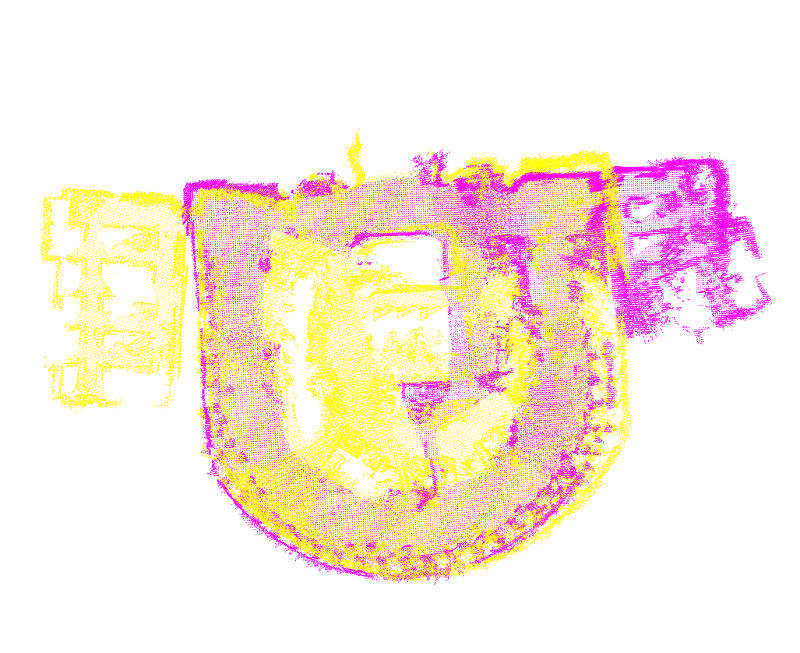
\includegraphics[width=4.53in]{../img/screenshot.jpg}
    \caption[The merged map for $2$ robots.]{Visualisation of registration between $2$ maps using a \texttt{map\_merge\_3d} package.}
    \label{fig:mapmergescreenshot}
\end{figure}

The \gls{ROS} node can merge maps from the arbitrary number of robots. It expects maps from individual robots as \gls{ROS} topics and does not impose any particular messaging between robots. If your run multiple robots under the same \gls{ROS} master then \texttt{map\_merge\_3d} may work for you out-of-the-box, this makes it easy to setup a simulation experiment.

In the multi-robot exploration scenario your robots probably run multiple \gls{ROS} masters and you need to setup a communication link between robots. Common solution might be \href{http://wiki.ros.org/multimaster_fkie}{multimaster\_fkie} package. You need to provide maps from your robots on local topics (under the same master). Also if you want to distribute merged map and \href{http://wiki.ros.org/tf}{tf} transformations back to robots your communication must take care of it.

\section{Architecture}

\texttt{map\_merge\_3d} finds robot maps automatically and new robots can be added to the system at any time. \gls{3D} maps are expected as \texttt{sensor\_msgs/PointCloud2}, other map messages are not supported.

\begin{figure}
    \centering
    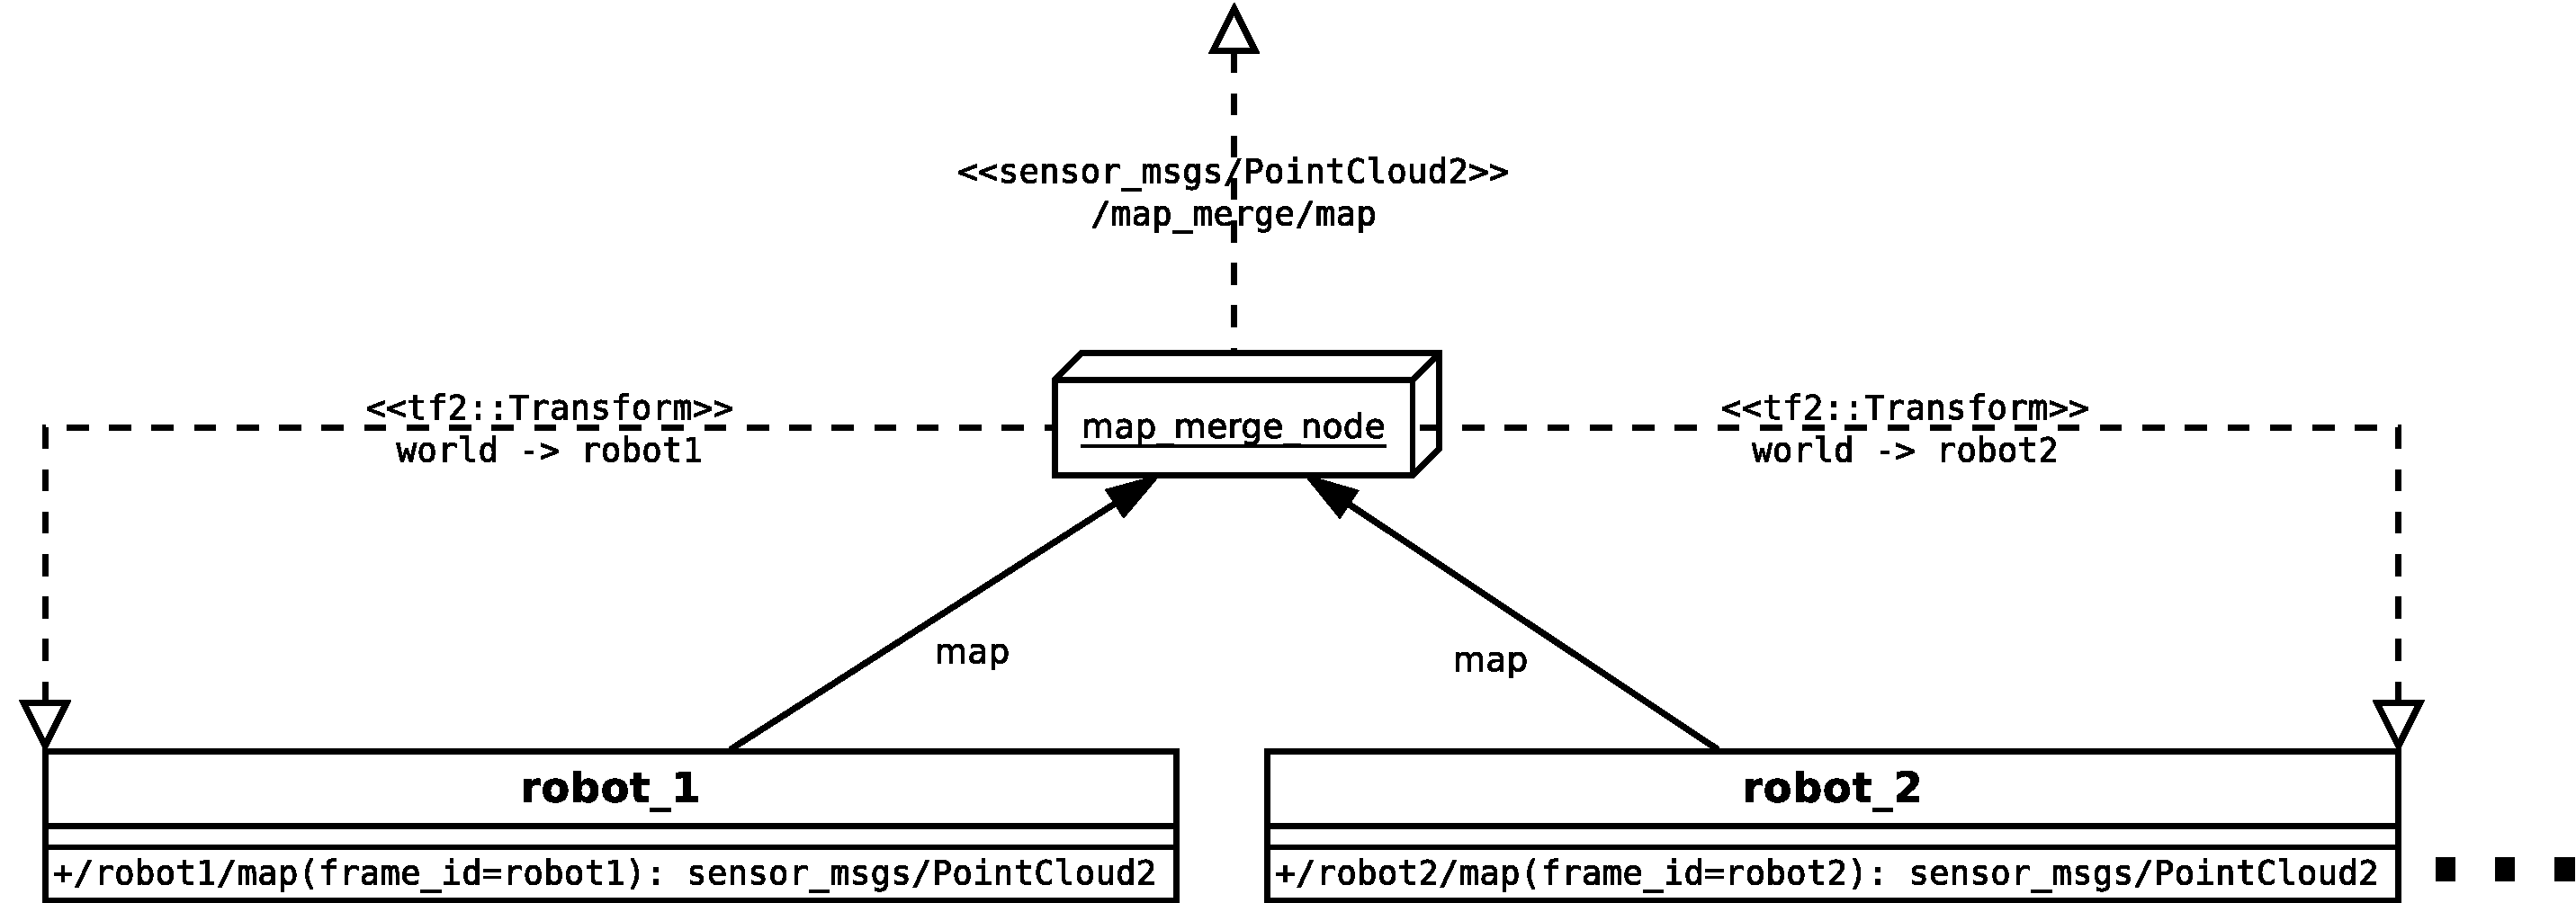
\includegraphics[width=\textwidth]{../img/architecture.pdf}
    \caption[The architecture of the \texttt{map\_merge\_node}]{Diagram showing \gls{ROS} \gls{API} of the map-merging node.}
    \label{fig:architecture}
\end{figure}

Recommended topics names for robot maps are \texttt{/robot1/map}, \texttt{/robot2/map} etc. However the names are configurable. All robots are expected to publish map under \texttt{<robot\_namespace>/map}, where topic name (\texttt{map}) is configurable, but must be the same for all robots. For each robot \texttt{<robot\_namespace>} is of cause different, but it does not need to follow any pattern. Further, you can exclude some topics using \texttt{robot\_namespace} parameter, to avoid merging unrelated point clouds.

\section{Estimation}

Transformations between maps are estimated by feature-matching algorithm and therefore it is required to have sufficient amount of overlapping space between maps to make a high-probability match. If maps don't have enough overlapping space to make a solid match, merger might reject those matches.

Estimating transforms between maps is cpu-intesive so you might want to tune \texttt{estimation\_rate} parameter to run the re-estimation less often.

\section{ROS API}

\subsection{map\_merge\_node}

Provides map merging services offered by this package. Dynamically looks for new robots in the system and merges their maps. Provides \texttt{tf} transforms.

\subsubsection{Subscribed Topics}

\ROStopic{<robot\_namespace>/map}{sensor\_msgs/PointCloud2}{Local map for a specific robot.}

\subsubsection{Published Topics}

\ROStopic{map}{sensor\_msgs/PointCloud2}{Merged map from all robots in the system.}

\subsubsection{Parameters}
\paragraph{Node Parameters}

Parameters affecting general setup of the node.

\ROSparam{\~{}robot\_map\_topic}{map}{string}{Name of robot map topic without namespaces (last component of the topic name). Only topics with this name are considered when looking for new maps to merge. This topics may be subject to further filtering (see below).}

\ROSparam{\~{}robot\_namespace}
{<empty string>}
{string}
{Fixed part of the robot map topic. You can employ this parameter to further limit which topics are considered during dynamic lookup for robots. Only topics which contain (anywhere) this string are considered for lookup. Unlike \texttt{robot\_map\_topic} you are not limited by namespace logic. Topics are filtered using text-based search. Therefore \texttt{robot\_namespace} does not need to be a \gls{ROS} namespace, but it can contain slashes etc. This string must be a common part of all maps topic name (all robots for which you want to merge map).}

\ROSparam{\~{}merged\_map\_topic}
{map}
{string}
{Topic name where merged map is published.}

\ROSparam{\~{}world\_frame}
{world}
{string}
{Frame id (in \href{http://wiki.ros.org/tf}{tf} tree) which is assigned to published merged map and used as reference frame for tf transforms.}

\ROSparam{\~{}compositing\_rate}
{0.3}
{double}
{Rate in Hz. Basic frequency on which the node merges maps and publishes merged map. Increase this value if you want faster updates.}

\ROSparam{\~{}discovery\_rate}
{0.05}
{double}
{Rate in Hz. Frequency on which this node discovers new robots (maps). Increase this value if you need more agile behaviour when adding new robots.}

\ROSparam{\~{}estimation\_rate}
{0.01}
{double}
{Rate in Hz. Frequency on which this node re-estimates transformations between maps. Estimation is cpu-intensive, so you may wish to lower this value.}

\ROSparam{\~{}publish\_tf}
{true}
{bool}
{Whether to publish estimated transforms in the \href{http://wiki.ros.org/tf}{tf} tree. See below.}

\paragraph{Registration Parameters}
\label{sec:registration-param}

Parameters affecting only registration algorithm used for estimating transformations between maps. These parameters should be defined in the same namespace as normal node parameters.

\ROSparam{\~{}resolution}
{0.1}
{double}
{Resolution used for the registration. Small value increases registration time.}

\ROSparam{\~{}descriptor\_radius}
{resolution * 8.0}
{double}
{Radius for descriptors computation.}

\ROSparam{\~{}outliers\_min\_neighbours}
{50}
{int}
{Minimum number of neighbours for a point to be kept in the map during outliers pruning.}

\ROSparam{\~{}normal\_radius}
{resolution * 6.0}
{double}
{Radius used for estimating normals.}

\ROSparam{\~{}keypoint\_type}
{SIFT}
{string}
{Type of keypoints used. Possible values are \gls{SIFT}, HARRIS.}

\ROSparam{\~{}keypoint\_threshold}
{5.0}
{double}
{Keypoints with lower response that this value are pruned. Lower this threshold when using Harris keypoints (you can set $0.0$).}

\ROSparam{\~{}descriptor\_type}
{PFH}
{string}
{Type of descriptors used. Possible values are \gls{PFH}, \gls{PFHRGB}, \gls{FPFH}, \gls{RSD}, \gls{SHOT}, \gls{SC3D}.}

\ROSparam{\~{}estimation\_method}
{MATCHING}
{string}
{Type of descriptors matching algorithm used. This algorithm is used for initial global match. Possible values are \texttt{MATCHING}, \texttt{SAC\_IA}.}

\ROSparam{\~{}refine\_transform}
{true}
{bool}
{Whether to refine estimated transformation with \gls{ICP} or not.}

\ROSparam{\~{}inlier\_threshold}
{resolution * 5.0}
{double}
{Inlier threshold used in \gls{RANSAC} during estimation.}

\ROSparam{\~{}max\_correspondence\_distance}
{inlier\_threshold * 2.0}
{double}
{Maximum distance for matched points to be considered the same point.}

\ROSparam{\~{}max\_iterations}
{500}
{int}
{Maximum iterations for \gls{RANSAC}.}

\ROSparam{\~{}matching\_k}
{5}
{int}
{Number of the nearest descriptors to consider for matching.}

\ROSparam{\~{}transform\_epsilon}
{1e-2}
{double}
{The smallest change allowed until \gls{ICP} convergence.}

\ROSparam{\~{}confidence\_threshold}
{0.0}
{double}
{Minimum confidence in the pair-wise transform estimate to be included in the map-merging graph. Pair-wise transformations with lower confidence are not considered when computing global transforms. Increase this value if you are having problems with invalid transforms being estimated. The confidence value is computed as a reciprocal of Euclidean distance between transformed maps.}

\ROSparam{\~{}output\_resolution}
{0.05}
{double}
{Resolution of the merged global map.}

\subsubsection{Provided tf Transforms}

\ROStransform{world}{mapX\_frame}
{Transformation from the world frame (which name can be configured using \texttt{world\_frame} parameter) to each of the maps. Each map must have a correct \texttt{frame\_id} set (instead \texttt{mapX\_frame}) in the \texttt{sensor\_msgs/PointCloud2} message. If the transformation could not be estimated, null transformation is published.}

\section{Tools}

Alongside \gls{ROS} node \texttt{map\_merge\_3d} provides command-line tools to work with point cloud maps saved in \texttt{pcd} files. Both tools accept any of the registration parameters described in section~\ref{sec:registration-param}.

The tools use \gls{PCL} command-line parsing module. \gls{PCL} command-line parsing has some limits (\gls{PCL} users won't be surprised): it supports only \texttt{--param value} format, \texttt{--param=value} is not accepted. Unknown options are ignored. Options may be arbitrarily mixed with filenames. There are no short versions for parameters.

\subsection{map\_merge\_tool}

Tool for merging maps offline. Produces \texttt{output.pcd} with merged global map. This tool can merge arbitrary number of maps.

\subsubsection{Usage}

\begin{code}
rosrun map_merge_3d map_merge_tool [--param value] map1.pcd
map2.pcd [map3.pcd...]
\end{code}

For example to use SHOT descriptors with 3 maps:

\begin{code}
rosrun map_merge_3d map_merge_tool --descriptor_type SHOT map1.pcd
map2.pcd map3.pcd
\end{code}

\subsection{registration\_visualisation}

Visualises pair-wise transform estimation between 2 maps. Uses \gls{PCL} visualiser for the visualisation.

\subsubsection{Usage}

\begin{code}
rosrun map_merge_3d registration_visualisation [--param value]
map1.pcd map2.pcd
\end{code}

After one step of the estimation a visualisation window appears. You can freely navigate the point cloud, save a screenshot or camera parameters (press \texttt{h} to see all shortcuts). After the window is closed, estimation continues with the next phase and the next visualisation window appears. Details about estimation progress are printed to \texttt{stdout}.

\section{Acknowledgements}

This package was developed as part of my master thesis at \href{http://www.mff.cuni.cz/to.en/}{Charles University} in Prague.
